\documentclass{beamer}

\usepackage{listings}
\lstset{language=C++,basicstyle=\footnotesize\ttfamily,breaklines=true}

% Setup appearance:

% \usetheme{Darmstadt}
% \usefonttheme[onlylarge]{structurebold}
% \setbeamerfont*{frametitle}{size=\normalsize,series=\bfseries}
\setbeamertemplate{navigation symbols}{}

\begin{document}

\begin{frame}{Recap}
  \begin{figure}[htbp]
  \centering
  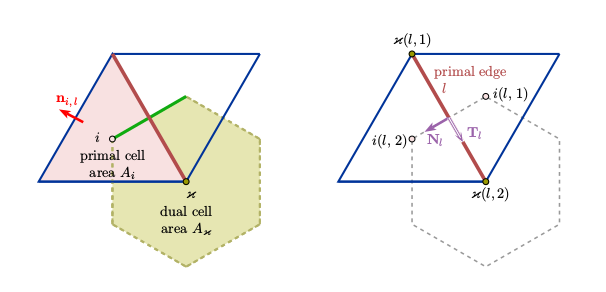
\includegraphics[width=0.8\textwidth]{1.png}
  \end{figure}
  \[\text{div}(v)_i = \frac{1}{A_i}\sum\limits_{l\in \mathcal{E}(i)}v_{n_l}(N_l \cdot n_{i,l})l\]
\end{frame}

\begin{frame}[fragile]{Recap}
  \begin{figure}[htbp]
  \centering
  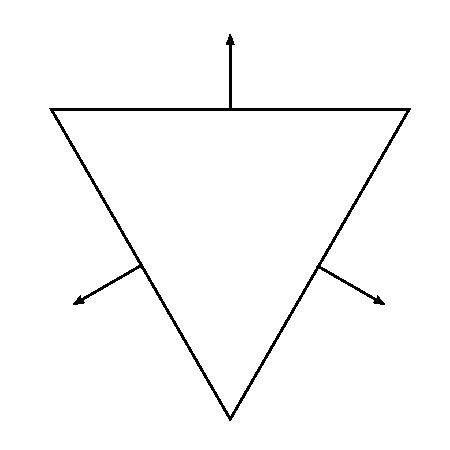
\includegraphics[width=0.2\textwidth]{flow_downward.pdf}
  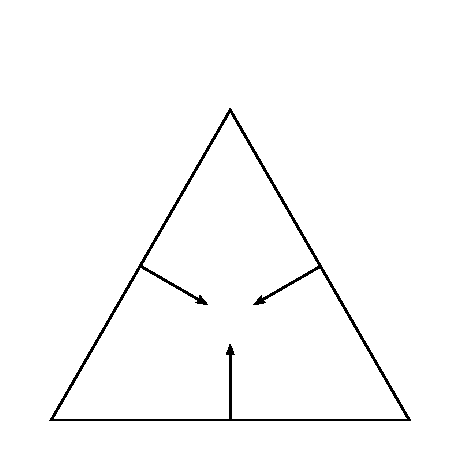
\includegraphics[width=0.2\textwidth]{flow_upward.pdf}
  \end{figure}
  \begin{align*}
    \text{div}(\bm{v})_i& = \frac{1}{A_i}\sum\limits_{l\in\mathcal{E}(i)}v_{n_l}l \quad \text{for downward cells}\\
    \text{div}(\bm{v})_i& = -\frac{1}{A_i}\sum\limits_{l\in\mathcal{E}(i)}v_{n_l}l \quad \text{for upward cells}
  \end{align*}
  \begin{lstlisting}[basicstyle=\scriptsize\ttfamily]
auto ff = [](const double _in1, const double _in2, const double _res) -> double
    { return _in1 * _in2 + _res; };
eval(out_cells()) =
    eval(on_edges(ff, 0.0, in_edges(), edge_length())) / eval(cell_area());
  \end{lstlisting}
\end{frame}

\begin{frame}{}
  From
  \begin{equation*}
    \text{div}(\bm{v})_i = \frac{1}{A_i}\sum\limits_{l\in\mathcal{E}(i)}v_{n_l}l
  \end{equation*}
  to
  \begin{equation*}
    \text{div}(v)_i
    &= \frac{1}{A_i}\sum\limits_{l\in \mathcal{E}(i)}v_{n_l}(N_l \cdot n_{i,l})l = \sum\limits_{l\in \mathcal{E}(i)}w_{i,l}v_{n_l}
  \end{equation*}
  \begin{itemize}
  \item One multiplication less. (Not necessarily faster)
  \item More general. (Definitely needed)
  \end{itemize}
\end{frame}

\begin{frame}{More operators}
  \begin{equation*}
    \text{div}(v)_i
    &= \frac{1}{A_i}\sum\limits_{l\in \mathcal{E}(i)}v_{n_l}(N_l \cdot n_{i,l})l = \sum\limits_{l\in \mathcal{E}(i)}w_{i,l}v_{n_l}
  \end{equation*}
  edge-to-cell averaging:
  \begin{equation*}
      \bar{\varrho}_i=\sum\limits_{l \in \mathcal{E}(i)}\frac{A_{i,l}}{A_i}\varrho_{l}= \sum\limits_{l\in \mathcal{E}(i)}w_{i,l}v_{n_l}
  \end{equation*}
  cell-to-edge averaging:
  \begin{equation*}
      \breve{\varrho}_l=\sum\limits_{j=1,2}\frac{A_{i(l,j)}}{A_l}\varrho_{i(l,j)}=\sum\limits_{j=1,2}w_{i(l,j)}\varrho_{i(l,j)}
  \end{equation*}
  Used in discretizing the pressure gradient force:
  \begin{equation*}
    \overline{\overline\psi}_l = \frac{A_{i(l,2),l}}{A_l}\psi_{i(l,1)} + \frac{A_{i(l,1),l}}{A_l}\psi_{i(l,2)}=\sum\limits_{j=1,2}w_{i(l,j)}\psi_{i(l,j)}
  \end{equation*}
\end{frame}

\begin{frame}[fragile]{Fields on multiple locations}
\texttt{\{i,c,j,k\}}

\texttt{\{i,c,j,k,extra\_dimension\}} (new!)

How to access:
\begin{lstlisting}
edges_of_cells_storage_type weights;
weights(i, c, j, k, 2);
\end{lstlisting}

In a functor:
\begin{lstlisting}
typedef in_accessor<1, icosahedral_topology_t::cells, extent<1>, 5 > weights;

using edge_of_cells_dim = dimension< 5 >;
edge_of_cells_dim::Index edge;
eval(weights(edge+2));
\end{lstlisting}
\end{frame}

\begin{frame}{Other than multiple-location \texttt{weights}}
  What else do we need?
  \[
  \text{div}(v)_i = \sum\limits_{l\in \mathcal{E}(i)}w_{i,l}v_{n_l}
  \]
  \texttt{on\_edges()} are currently not dealing with multiple-location fields. We need to fold manually. But when we use \texttt{eval(weights(edge+0))} to get $w_{i,0}$, how do we get $v_{n_0}$?

  $\rightarrow$ expose topology to user

  $\rightarrow$ fix neighbors order
\end{frame}

\begin{frame}[fragile]{Expose topology to user}
  \begin{lstlisting}
/*
 * this stencil is primarily on cells
 */

typedef in_accessor<0, icosahedral_topology_t::edges, extent<1> > in_edges;

auto neighbors_offsets = connectivity< cells , edges >::offsets(eval.position()[1]);

// get the first edge on cell
eval(in_edges(neighbor_offsets[0]));

// iterate over all edges of cell
for (auto neighbor_offset : neighbors_offsets)
  eval(in_edges(neighbor_offset));
  \end{lstlisting}
\end{frame}

\begin{frame}[fragile]{Fix neighbors order}
  \begin{lstlisting}
Neighbor edges of a cell must follow the same convention than neighbor cells of a cell.
I.e. the following
          /\
         1  2
        /_0__\
 imposes
      ____________
      \    /\    /
       \1 /  \2 /
        \/____\/
         \  0 /
          \  /
           \/
  \end{lstlisting}
  Now \texttt{eval(weights(edge+0))} and \texttt{eval(in\_edges(neighbor\_offsets[0]))} point to the same direction.
\end{frame}

\begin{frame}[fragile]{Combining everything, now a div}
\begin{lstlisting}[basicstyle=\scriptsize\ttfamily]
template<typename Evaluation>
GT_FUNCTION static void Do(Evaluation const &eval, x_interval)
{
    typedef typename icgrid::get_grid_topology< Evaluation >::type grid_topology_t;

    // for multiple-location fields
    using edge_of_cells_dim = dimension< 5 >;
    edge_of_cells_dim::Index edge;

    // for exposed topology
    auto neighbors_offsets = connectivity< cells , edges >::offsets(eval.position()[1]);

    eval(out_cells()) = 0.;
    ushort_t e=0;
    for (auto neighbor_offset : neighbors_offsets) {
        eval(out_cells()) += eval(in_edges(neighbor_offset)) * eval(weights(edge+e));
        e++;
    }
}
\end{lstlisting}

  We will discuss how to make this look better later.
\end{frame}

\begin{frame}{grad}
  \begin{figure}[htbp]
  \centering
  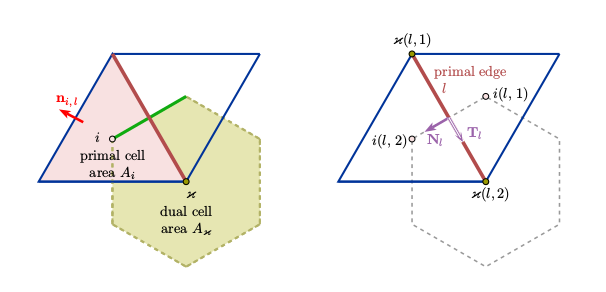
\includegraphics[width=0.8\textwidth]{1.png}
  \end{figure}
  \[\text{grad}_n(\varrho)_l = \frac{\varrho_{i(l,2)}-\varrho_{i(l,1)}}{\hat{l}}\]

  $\rightarrow$ fix neighbour order
\end{frame}

\begin{frame}[fragile]{Neighbors order}
  \begin{figure}[htbp]
  \centering
  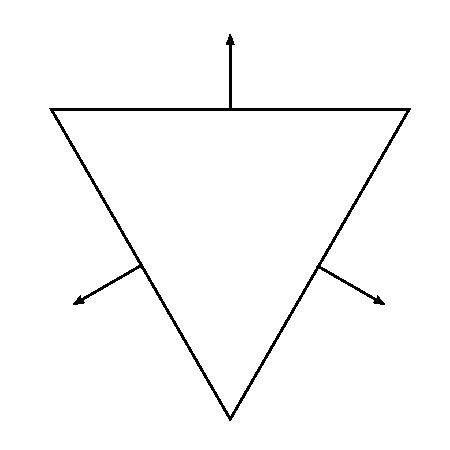
\includegraphics[width=0.2\textwidth]{flow_downward.pdf}
  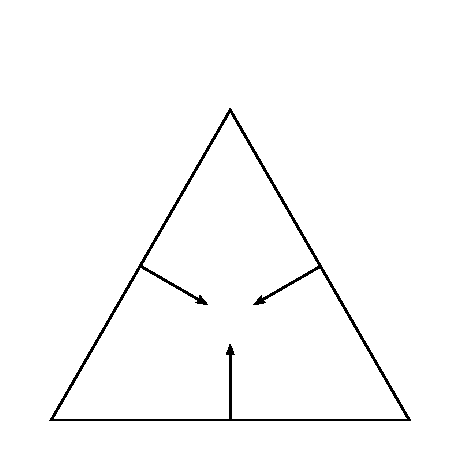
\includegraphics[width=0.2\textwidth]{flow_upward.pdf}
  \end{figure}

  Cell neighbours of an edge, in the order $0 \rightarrow 1$ follow the direction of the $N_l$.
  \begin{lstlisting}
            neighbors order
                              /\
                  ______     / 0\    ______
                 /\  1 /    /____\   \ 1  /\
                /0 \  /     \    /    \  / 0\
               /____\/       \1 /      \/____\
                              \/
  \end{lstlisting}
\end{frame}

\begin{frame}[fragile]{Neighbors order}
  \begin{figure}[htbp]
  \centering
  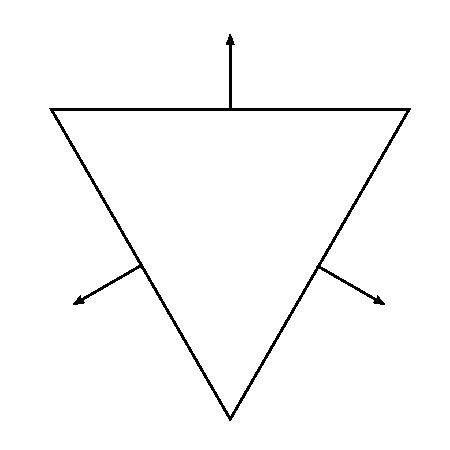
\includegraphics[width=0.2\textwidth]{flow_downward.pdf}
  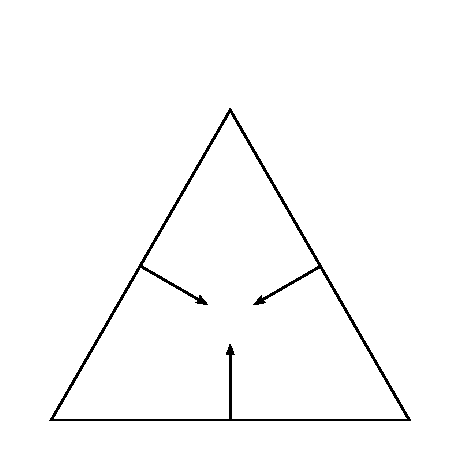
\includegraphics[width=0.2\textwidth]{flow_upward.pdf}
  \end{figure}

  Vertex neighbors of an edge, in the order $0 \rightarrow 1$ defines a vector $N_l$ which is perpendicular to $N_t$.
  \begin{lstlisting}
            neighbors order
                 1______      /\      ______0
                 /\    /     /  \     \    /\
                /  \  /    0/____\1    \  /  \
               /____\/      \    /      \/____\
                     0       \  /       1
                              \/
  \end{lstlisting}

  Useful for
  \[\text{grad}_{\tau}(\varrho)_l = \frac{\varrho_{\varkappa(l,2)}-\varrho_{\varkappa(l,1)}}{l}\]
\end{frame}

\begin{frame}{Neighbors order}
  We also set rules for neighbors of vertexes. Helpful for a curl.
\end{frame}

\begin{frame}[fragile]{A grad}
  \[\text{grad}_n(\varrho)_l = \frac{\varrho_{i(l,2)}-\varrho_{i(l,1)}}{\hat{l}}\]

  \begin{lstlisting}[basicstyle=\scriptsize\ttfamily]
typedef in_accessor<0, icosahedral_topology_t::cells, extent<1> > in_cells;
typedef in_accessor<1, icosahedral_topology_t::edges, extent<1> > dual_edge_length;
typedef inout_accessor<2, icosahedral_topology_t::edges> out_edges;

template<typename Evaluation>
GT_FUNCTION static void Do(Evaluation const &eval, x_interval) {
    auto neighbors_offsets =
      connectivity<edges, cells>::offsets(eval.position()[1]);

    eval(out_edges()) =
      ( eval(in_cells(neighbors_offsets[0])) -
        eval(in_cells(neighbors_offsets[1]))
      ) / eval(dual_edge_length());
}
  \end{lstlisting}
\end{frame}

\begin{frame}{Evaluation}
\end{frame}

\begin{frame}{Syntactic sugar}
\end{frame}

\begin{frame}{Next}
  \begin{itemize}
    \item Roofline model
    \item Evaluate on GPU
    \item Mass flux divergence:
      \begin{equation*}
        \text{div}(\bm{v}\Delta p)_{i, k}=\frac{1}{A_i} \sum\limits_{l\in\mathcal{E}(i)}v_{n_l,k}\Delta\breve{p}_{l,k}(\bm{N}_l\cdot\bm{n}_{i,l})l
      \end{equation*}
      \begin{itemize}
        \item fuse of operators: cell-to-edge averaging and div
        \item k level: $\Delta p_k = \frac{1}{2}(p_{k-1/2}+p_{k+1/2})$
      \end{itemize}
  \end{itemize}
\end{frame}
\end{document}
